\chapter{Prérequis}

\section{Principe des tests d’hypothèse}
On  étudie  une  population  dont  les  éléments  possèdent  un  caractère  (mesurable  ou qualitatif) et dont la valeur du paramètre relative au caractère étudié est inconnue. Une  hypothèse  est  formulée  sur  la  valeur  du  paramètre  :  cette  formulation  résulte  de considérations  théoriques,  pratiques  ou  encore  elle  est  simplement  basée  sur  un pressentiment. Pour  décider  si  l’hypothèse  formulée  est  supportée  ou  non  par  les observations,  il  faut  une  méthode  qui  permettra  de  conclure  si  l’écart  observé  entre  la valeur  de  la  statistique  obtenue  dans  l’échantillon  et  celle  du  paramètre  spécifié  dans l’hypothèse  est  trop  important  pour  être  uniquement  imputable  au  hasard  de l’échantillonnage.

On part d'une hypothèse nulle \textbf{H0}(figure \ref{fig:H0}) et on va vérifier si on peut la rejeter ou pas.
\begin{figure}[H]
    \centering
    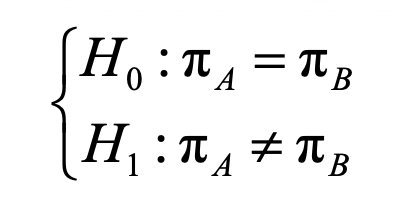
\includegraphics{images/H0.png}
    \caption{Test statistique}
    \label{fig:H0}
\end{figure}
On va aussi définir $\delta = \pi_{A}-\pi_{B}$ qui est l'\textbf{effet du traitement}.\\
On réalise nos expériences sur des échantillons de la population. Dans notre cas, un groupe A qui va recevoir un traitement A et un groupe B qui va recevoir un traitement B. On définit donc aussi :
$P_{A}$ : taux de succès avec le traitement A 
$P_{B}$ : taux de succès avec le traitement B. 
\subsection{Erreur de type I et erreur de type II}
Lorsqu'rejette H0 ou pas, on a deux types d'erreurs possibles 
\begin{figure}[H]
    \centering
    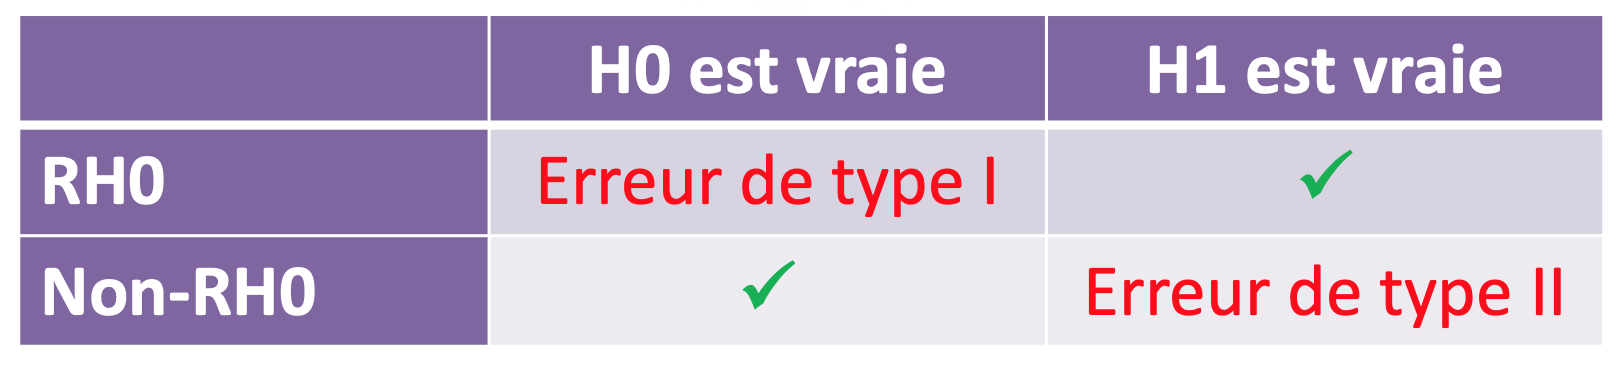
\includegraphics[scale =0.5]{images/errors.png}
    \caption{Deux types d'erreur}
    \label{fig:type_error}
\end{figure}

\subsubsection{Erreur de type I}
Conclure qu’il y a un effet du traitement ($\pi_{A} \neq \pi_{B}$) alors qu’en fait il n’y en a pas($\pi_{A} = \pi_{B}$) =\textbf{faux-positif}

\subsubsection{Erreur de type II}
Conclure qu’il n’y a pas d’effet du traitement ($\pi_{A} = \pi_{B}$) alors qu’en fait il y en a un($\pi_{A} \neq \pi_{B}$) = \textbf{Faux-négatif}

\subsection{Puissance d'un test}
On va plus souvent parler de la puissance d’un test : 
$$Puissance = 1 - \beta$$

plutôt que du risque d’erreur de type II ($\beta$), ce qui est en fait équivalent.\\
$$\beta = P(NRH_{0},H_{1})$$ et $$puissance = P(RH_{0},H_{1})$$

Ainsi, la puissance est la probabilité de rejeter $H0$ si $H1$ est vrai.

\subsection{Test bilatéral versus test unilatéral}

\section{Endpoint binaire}

\begin{figure}[H]
    \centering
    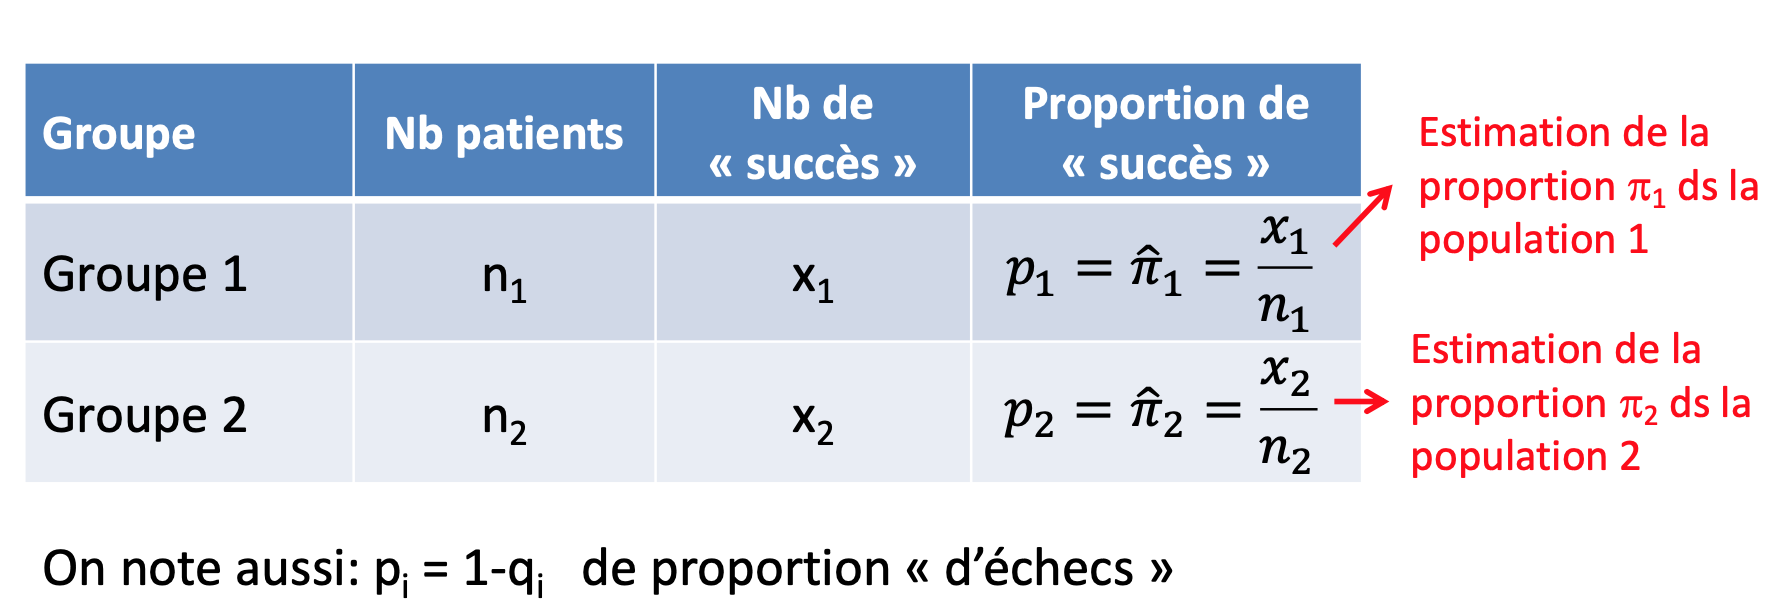
\includegraphics[scale = 0.3]{images/estimationproportion.png}
    \caption{Tableau endpoint binaire}
    \label{fig:my_label}
\end{figure}

Pour calculer de l’intervalle de confiance pour l’estimation d’une probabilité (proportion) sur base de l’approximation normale de la binomiale (sans correction) :
\begin{figure}[H]
    \centering
    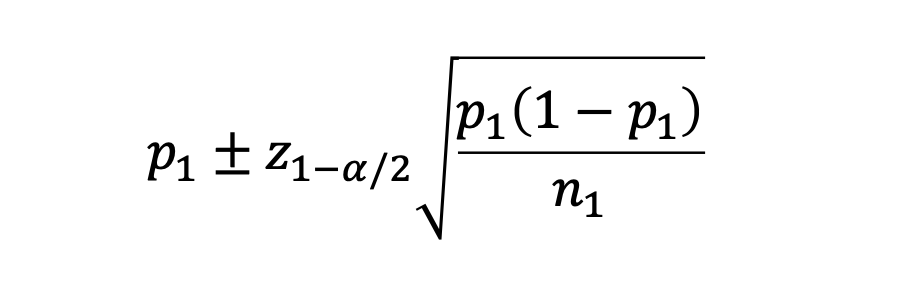
\includegraphics[scale = 0.5]{images/intervalprob.png}
    \caption{intervalle de confiance d'une probabilité (proportion)}
    \label{fig:my_label}
\end{figure}

\begin{figure}[H]
    \centering
    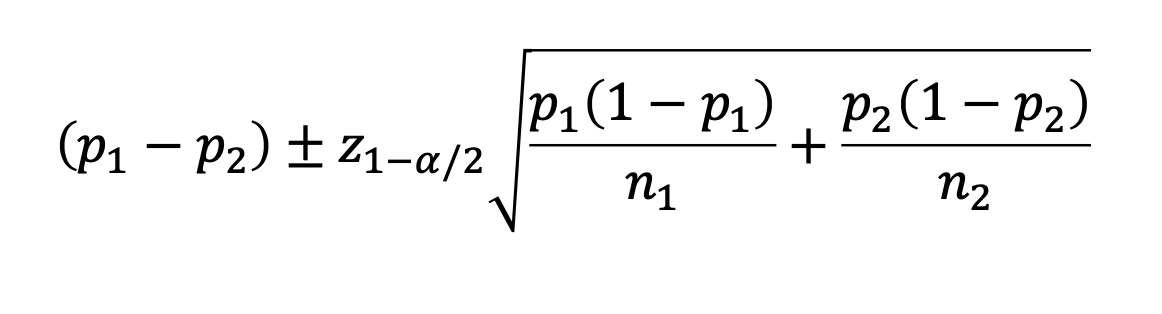
\includegraphics[scale = 0.5]{images/intervaldiffprop.png}
    \caption{intervalle de confiance pour la différence de deux proportions}
    \label{fig:my_label}
\end{figure}


\section{Endpoint continu}
\subsection{Premier cas $\sigma_1^2 \neq \sigma_2^2$}
\begin{figure}[H]
    \centering
    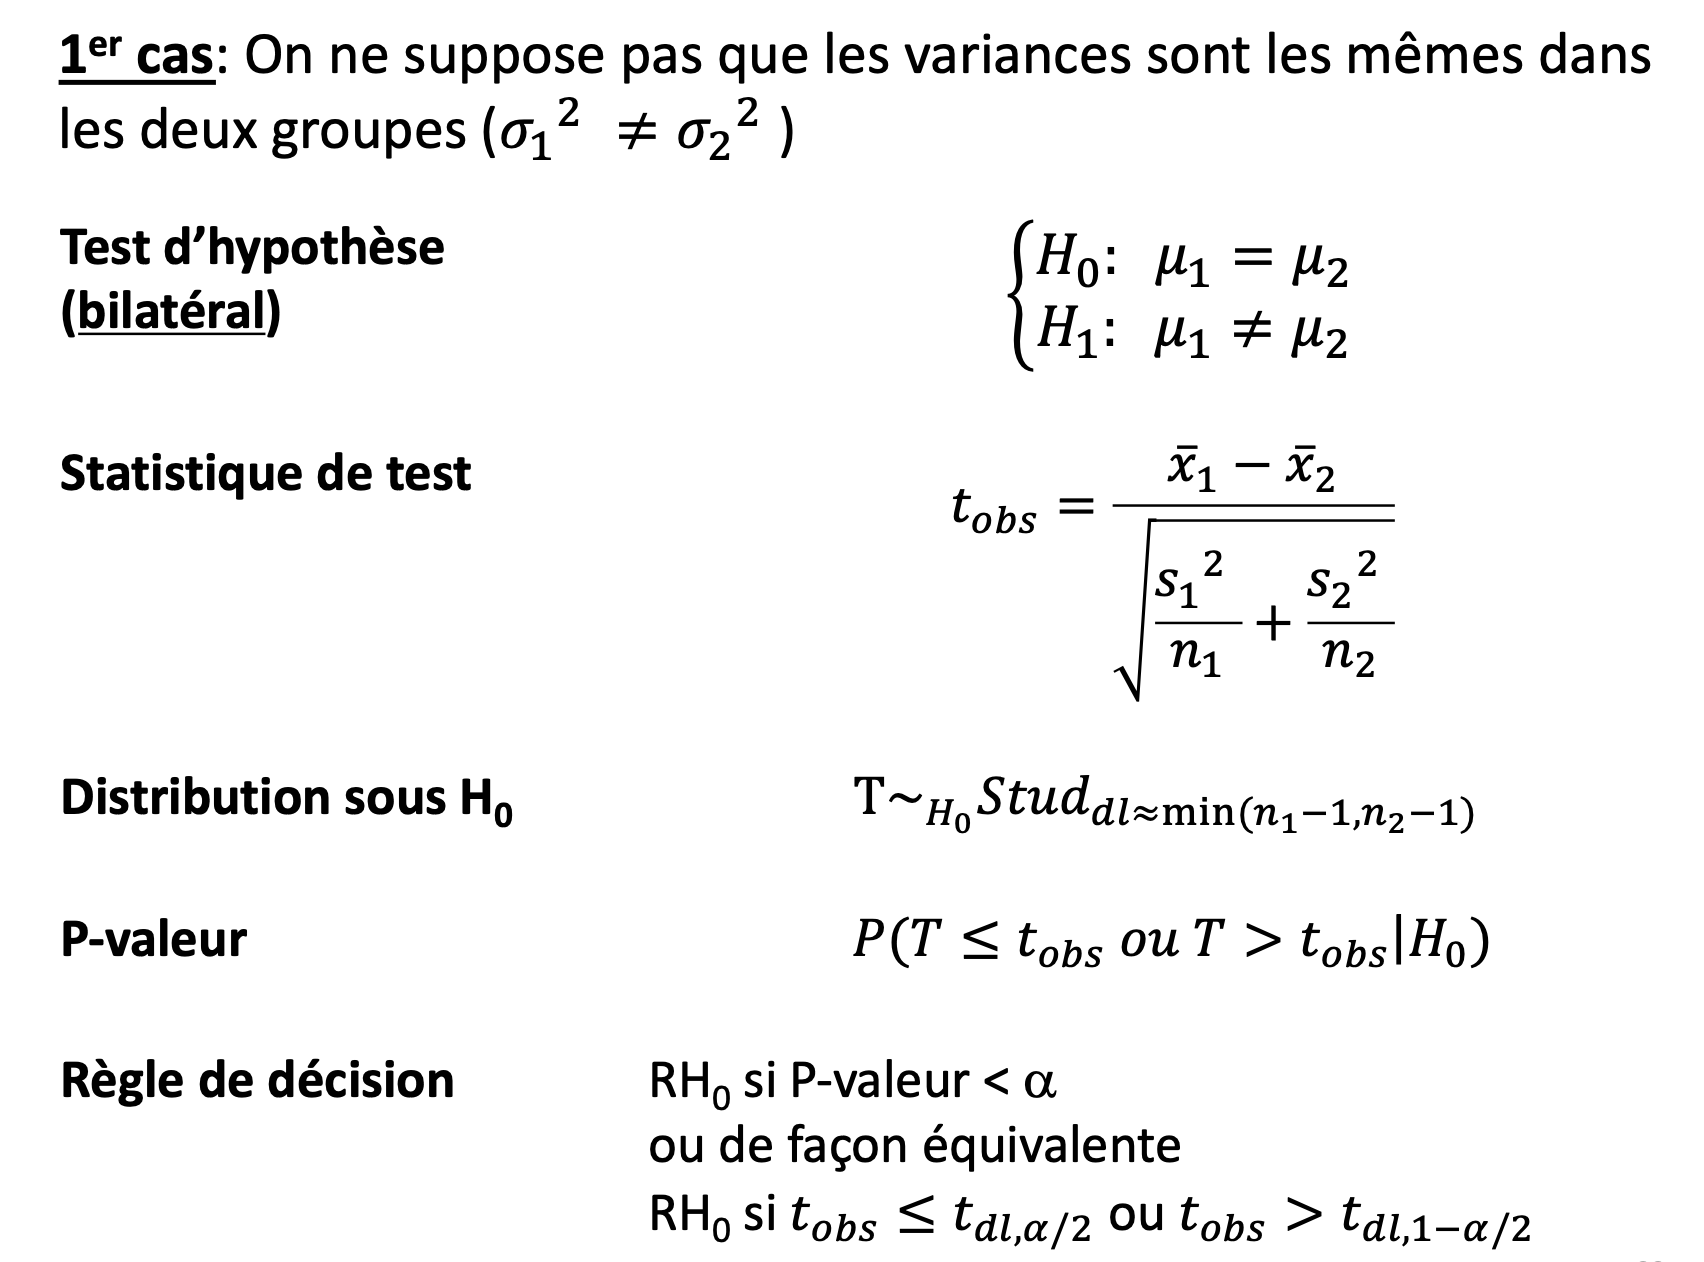
\includegraphics[scale = 0.5]{images/firstcasecontinu.png}
    \caption{Premier cas $\sigma_1^2 \neq \sigma_2^2$}
    \label{fig:my_label}
\end{figure}

\subsection{Deuxième cas $\sigma_1^2 = \sigma_2^2$}
\begin{figure}[H]
    \centering
    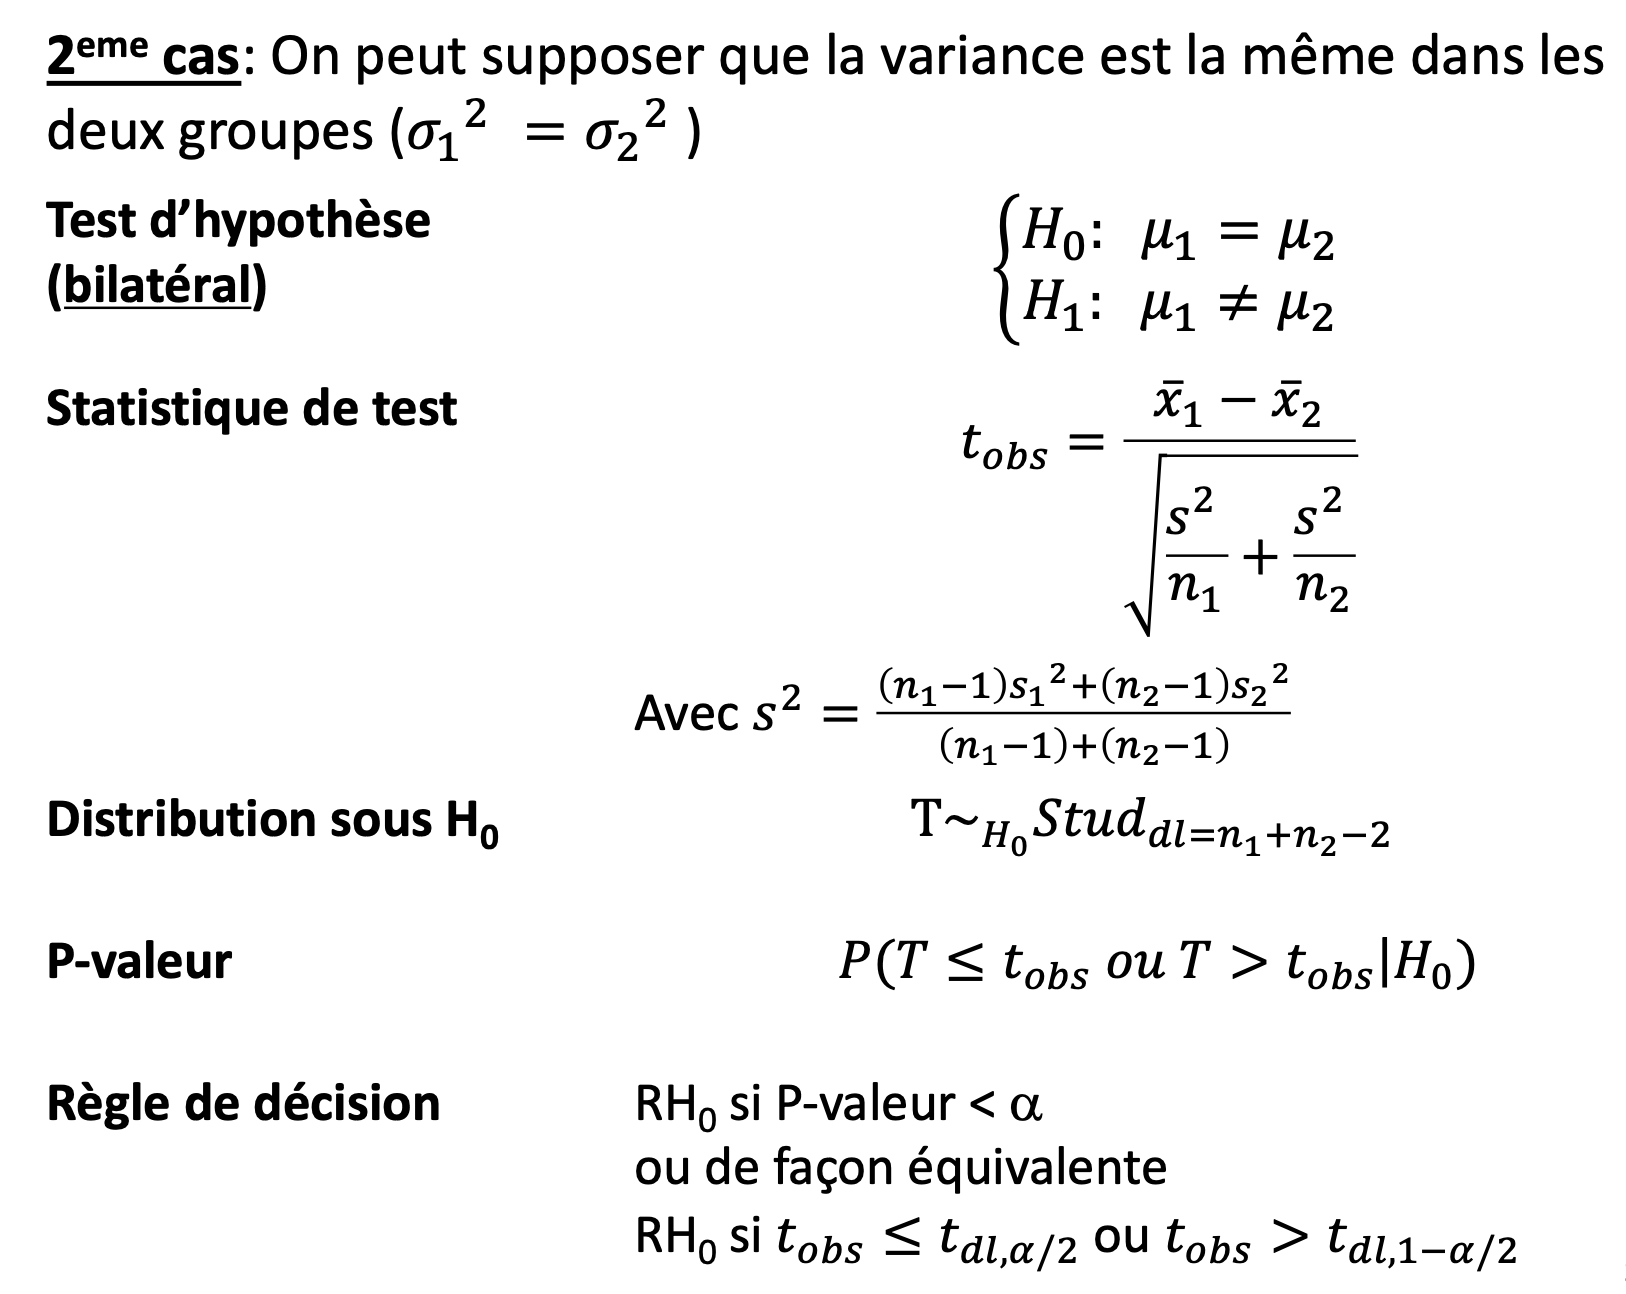
\includegraphics[scale = 0.5]{images/deuxiemecascontinu.png}
    \caption{Deuxième cas $\sigma_1^2 = \sigma_2^2$}
    \label{fig:my_label}
\end{figure}

